\documentclass[10pt,aspectratio=169]{beamer}
\usetheme[progressbar=frametitle,numbering=fraction]{metropolis}
\usepackage[T1]{fontenc}
\usepackage[utf8]{inputenc}
\usepackage[french]{babel}
\usepackage{booktabs}
\usepackage{tikz}
\usetikzlibrary{arrows.meta,positioning,shapes.geometric,calc,decorations.pathmorphing}
\usepackage{fontawesome5}
\graphicspath{{../../results/figures/}}

\definecolor{Lband}{HTML}{2CA02C}
\definecolor{Cband}{HTML}{9467BD}
\definecolor{cut}{HTML}{D62728}
\definecolor{ctrl}{HTML}{1F77B4}
\setbeamercolor{alerted text}{fg=cut}
\newcommand{\Lb}[1]{\textcolor{Lband}{\textbf{#1}}}
\newcommand{\Cb}[1]{\textcolor{Cband}{\textbf{#1}}}

\title{Bande L (NISAR) contre bande C (Sentinel-1)\\pour détecter une coupe rase en forêt vosgienne}
\subtitle{Test de faisabilité à l'appui de ma candidature au stage SERTIT / ICube\\
\small « Exploration des bandes L et P pour la détection de la déforestation et des glissements de terrain »}
\author{Mamadou Galy Diallo}
\date{Novembre 2026}

\begin{document}

\maketitle

%---------------------------------------------------------------------
\begin{frame}{En une phrase}
\centering
\Large
Sur une coupe rase réelle de 2,4~ha (Vosges, août 2026), la \Lb{cohérence interférométrique en bande L}
sépare la coupe de la forêt presque parfaitement (\Lb{AUC 0,995}), là où la \Cb{bande C} n'y parvient pas
(\Cb{AUC 0,74}).

\vspace{0.8em}
\normalsize
\begin{columns}[T]
\column{0.32\textwidth}\centering
\faSatellite\quad\textbf{Données réelles}\\[0.2em]
\small NISAR L2 (ISCE3), 3~géométries\\13 dates Sentinel-1
\column{0.32\textwidth}\centering
\faCogs\quad\textbf{Chaîne reproductible}\\[0.2em]
\small paquet Python + graphes SNAP\\tables générées automatiquement
\column{0.32\textwidth}\centering
\faBalanceScale\quad\textbf{Évaluation honnête}\\[0.2em]
\small contrôle avant coupe, bootstrap,\\comparaison à géométrie égale
\end{columns}
\end{frame}

%---------------------------------------------------------------------
\section{Contexte et question}

\begin{frame}{Pourquoi ce test ?}
\begin{columns}[T]
\column{0.55\textwidth}
\begin{itemize}
\item Le suivi radar des coupes repose aujourd'hui sur la \Cb{bande C} (Sentinel-1, alertes de type RADD,
  méthode des ombres).
\item Depuis 2025, \Lb{NISAR} (NASA-ISRO) fournit pour la première fois de la \Lb{bande L} gratuite et
  systématique sur l'Europe. Ses produits L2 sont générés par \textbf{ISCE3}.
\item \textbf{ROSE-L} (Copernicus, lancement prévu en 2028) assurera ensuite la bande L européenne.
\item \textbf{BIOMASS} (bande P) n'acquiert pas sur l'Europe de l'Ouest (zone d'exclusion SOTR) : c'est une
  perspective.
\end{itemize}
\column{0.42\textwidth}
\begin{block}{Question}
Sur une coupe rase récente des Vosges, la cohérence et la rétrodiffusion \Lb{NISAR} séparent-elles mieux la
coupe de la forêt intacte que \Cb{Sentinel-1} ?
\end{block}
\begin{alertblock}{Enjeu pour le stage}
Préparer une chaîne en bande L transposable à ROSE-L.
\end{alertblock}
\end{columns}
\end{frame}

\begin{frame}{La physique attendue}
\begin{columns}[c]
\column{0.52\textwidth}
\begin{tikzpicture}[scale=0.85]
  % ground
  \fill[brown!30] (0,0) rectangle (8,0.3);
  % trees
  \foreach \x in {0.8,2.3,3.8} {
    \fill[brown!70!black] (\x-0.08,0.3) rectangle (\x+0.08,2.4);
    \fill[green!50!black,opacity=0.75] (\x,2.9) ellipse (0.65 and 0.9);
  }
  % clear-cut
  \foreach \x in {5.2,6.1,7.0} { \fill[brown!60!black] (\x-0.15,0.3) rectangle (\x+0.15,0.45); }
  \node[font=\scriptsize] at (6.1,0.75) {coupe : sol nu, rémanents};
  % C band arrow
  \draw[-{Latex},very thick,Cband,decorate,decoration={snake,amplitude=1.2pt,segment length=4pt}] (1.0,5.2) -- (2.2,3.4);
  \node[Cband,font=\scriptsize\bfseries] at (0.7,5.45) {C, 5,6 cm};
  \node[Cband,font=\scriptsize,align=right,anchor=east] at (1.45,3.9) {s'arrête\\au feuillage};
  % L band arrow
  \draw[-{Latex},very thick,Lband,decorate,decoration={snake,amplitude=2.2pt,segment length=9pt}] (2.9,5.2) -- (3.75,1.2);
  \node[Lband,font=\scriptsize\bfseries] at (3.4,5.45) {L, 24 cm};
  \node[Lband,font=\scriptsize,align=left,anchor=west] at (4.55,2.0) {atteint troncs\\et branches};
\end{tikzpicture}
\column{0.46\textwidth}
\small
\begin{description}
\item[H1] Forêt intacte : cohérence à 12~j plus élevée en \Lb{L} qu'en \Cb{C} (troncs stables / feuilles mobiles).
\item[H2] Donc un contraste de cohérence coupe / forêt plus fort en \Lb{L}.
\item[H3] Une baisse de rétrodiffusion plus forte en \Lb{L} (la bande C sature sur forêt dense).
\item[H4] HV (polarisation croisée, diffusion de volume) est l'indicateur de rétrodiffusion le plus sensible.
\end{description}
\vspace{0.3em}
\footnotesize Hypothèses fixées \emph{avant} les calculs, à l'étape de cadrage.
\end{columns}
\end{frame}

\begin{frame}{Les deux grandeurs radar utilisées}
\begin{columns}[T]
\column{0.48\textwidth}
\begin{block}{Rétrodiffusion $\gamma^0$ (dB)}
Énergie renvoyée vers le radar, normalisée et corrigée du relief (RTC).
\begin{itemize}\small
\item HH, VV : co-polarisation (surface, double rebond).
\item HV, VH : polarisation croisée, sensible à la \textbf{diffusion de volume}, donc à la biomasse.
\end{itemize}
\end{block}
\column{0.48\textwidth}
\begin{block}{Cohérence interférométrique $\gamma$ (0--1)}
\[
\gamma=\frac{|\langle s_1 s_2^*\rangle|}{\sqrt{\langle|s_1|^2\rangle\langle|s_2|^2\rangle}}
\]
\small Ressemblance entre deux images prises à 12~jours d'écart : proche de 1 si la scène n'a pas bougé, proche
de 0 si elle a changé (feuilles, vent, coupe\ldots).
\end{block}
\end{columns}
\vspace{0.5em}
\centering\small Une coupe se voit de deux façons : \textbf{l'état change} ($\gamma^0$ baisse) et \textbf{l'événement
décorrèle} la paire qui l'encadre (cohérence basse).
\end{frame}

%---------------------------------------------------------------------
\section{Données et site}

\begin{frame}{Données et ingénierie de l'accès}
\footnotesize
\begin{tabular}{@{}lll@{}}
\toprule
& \Lb{NISAR (L, 1,26 GHz)} & \Cb{Sentinel-1 (C, 5,4 GHz)} \\
\midrule
Produits & L2 GCOV ($\gamma^0$ HH, HV) + GUNW (cohérence HH), ISCE3 & IW SLC (VV+VH), SNAP 14 \\
Géométries & A144, A72 (montantes), D138 (descendante) & orbite D139 (descendante), IW2 \\
Dates & 10--11 GCOV, 8--9 GUNW par géométrie & 13 dates, 14/06 $\to$ 06/11/2026 \\
Paires & 12~j ; \textbf{24~j sur la coupe} (acquisition manquante) & 12~j \\
\bottomrule
\end{tabular}

\vspace{0.4em}
\begin{columns}[T]
\column{0.48\textwidth}
\begin{exampleblock}{Lecture à distance NISAR}
HDF5 découpé en blocs $512\times512$ : lecture HTTPS des seuls blocs du site.
\textbf{15~s par couche au lieu de 20~min par fichier.}
\end{exampleblock}
\column{0.48\textwidth}
\begin{exampleblock}{SAFE Sentinel-1 réduits}
Lecture du zip distant par requêtes partielles : sous-fauchée IW2 seulement.
\textbf{1,6~Go au lieu de 4,6~Go par date.}
\end{exampleblock}
\end{columns}
\vspace{0.3em}
\centering\footnotesize Volume total évité : environ 30~h de téléchargement à 1,8~Mo/s.
\end{frame}

\begin{frame}{Trouver une vraie coupe : 16 candidats, 1 retenu}
\begin{columns}[c]
\column{0.58\textwidth}
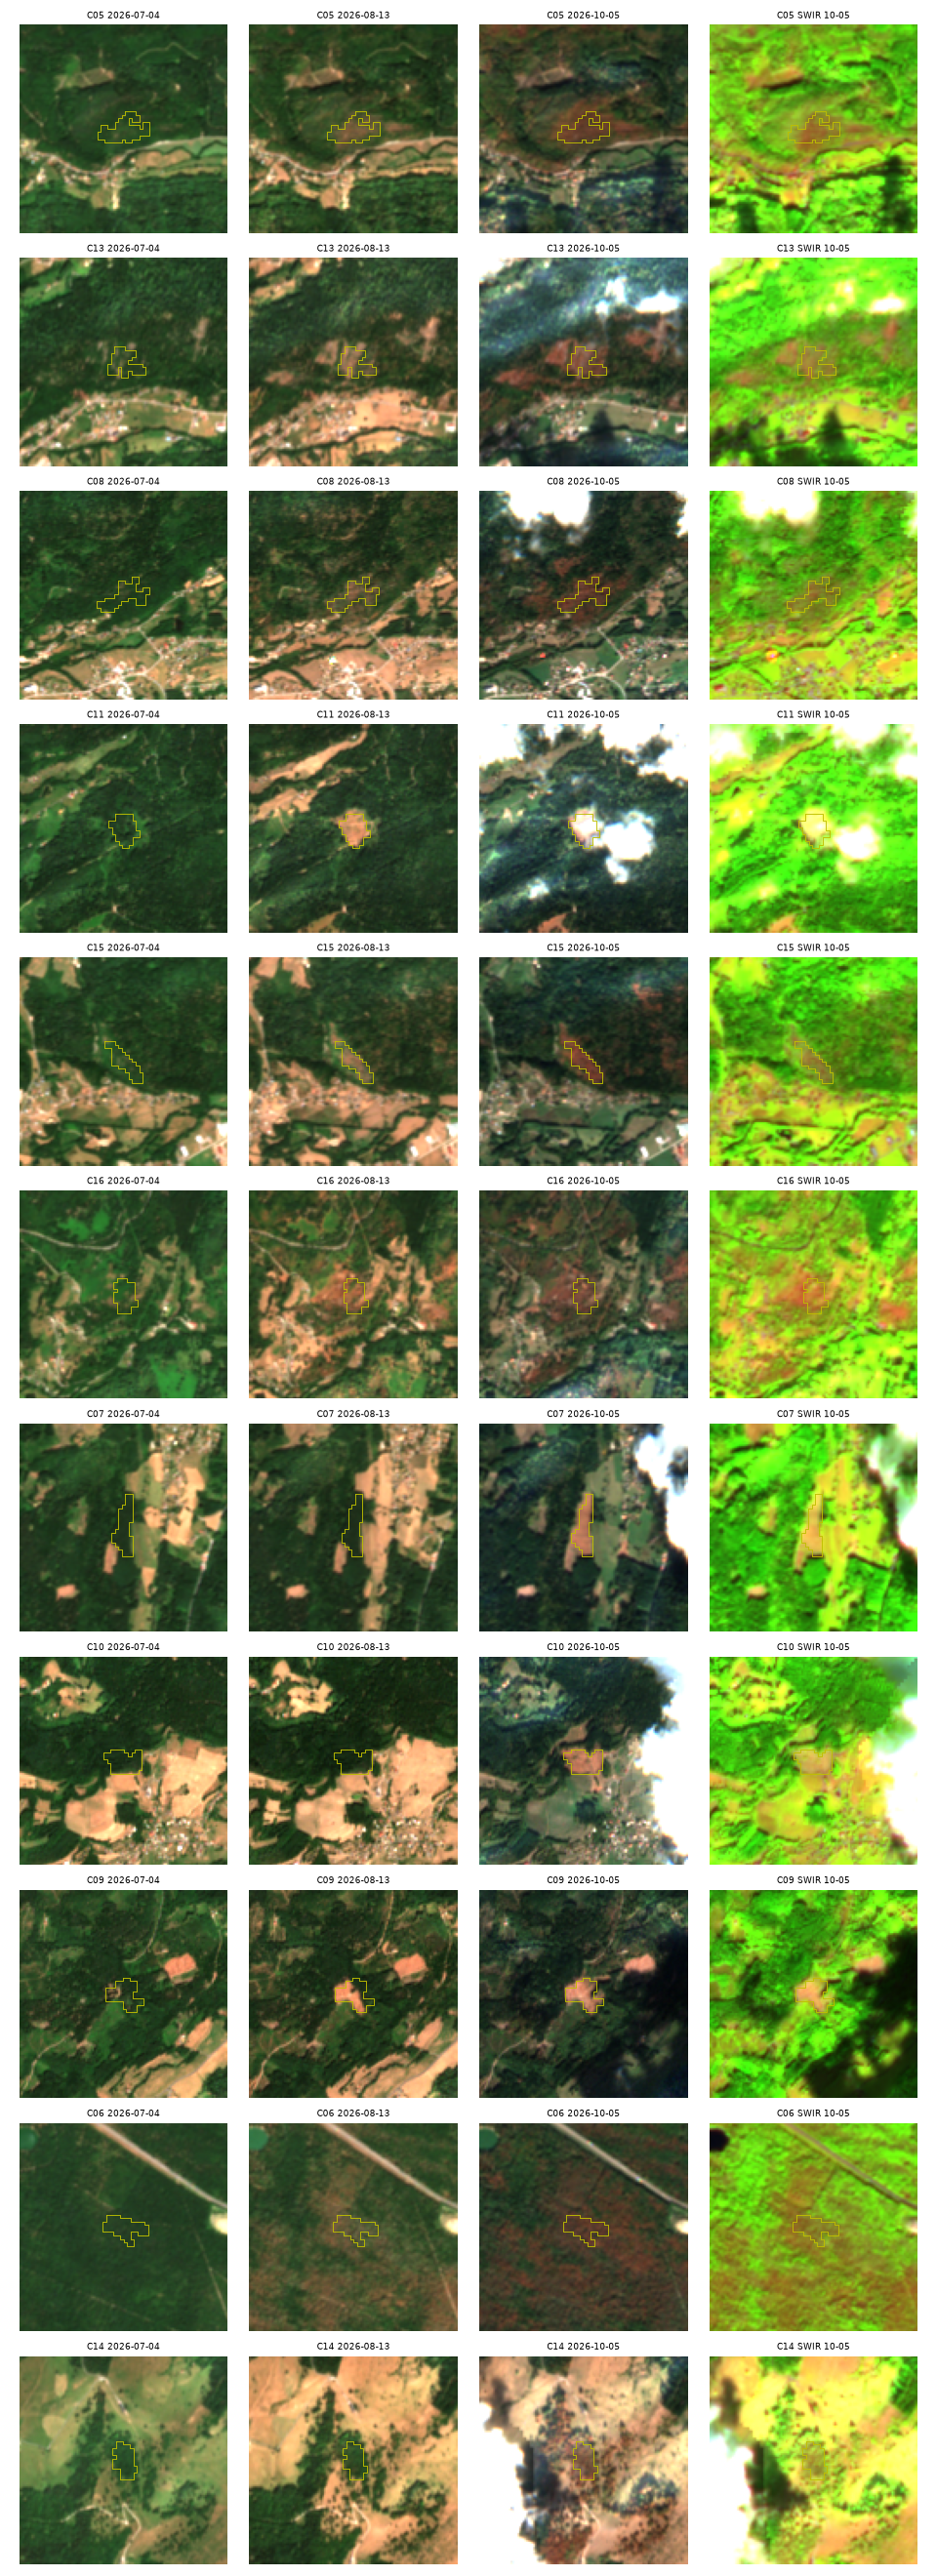
\includegraphics[width=\linewidth,height=0.8\textheight,keepaspectratio]{candidates_rgb_quicklooks.png}
\column{0.40\textwidth}
\small
\begin{enumerate}
\item Détection Sentinel-2 : NDVI avant $\geq 0{,}7$, dNDVI $\leq -0{,}3$, masque forêt WorldCover, $\geq 2$~ha.
\item Vérification par séries temporelles.
\item \textbf{Contrôle visuel} (couleurs vraies et SWIR) :
\begin{itemize}\footnotesize
\item 7 dépérissements (scolytes, sécheresse) ;
\item étangs, lisières, ripisylve ;
\item \textbf{C11 : vraie coupe rase} au sein d'une forêt continue.
\end{itemize}
\end{enumerate}
\footnotesize Leçon : un seuil NDVI seul confond coupe et dépérissement.
\end{columns}
\end{frame}

\begin{frame}{Site C11 et forêt témoin}
\begin{columns}[c]
\column{0.62\textwidth}
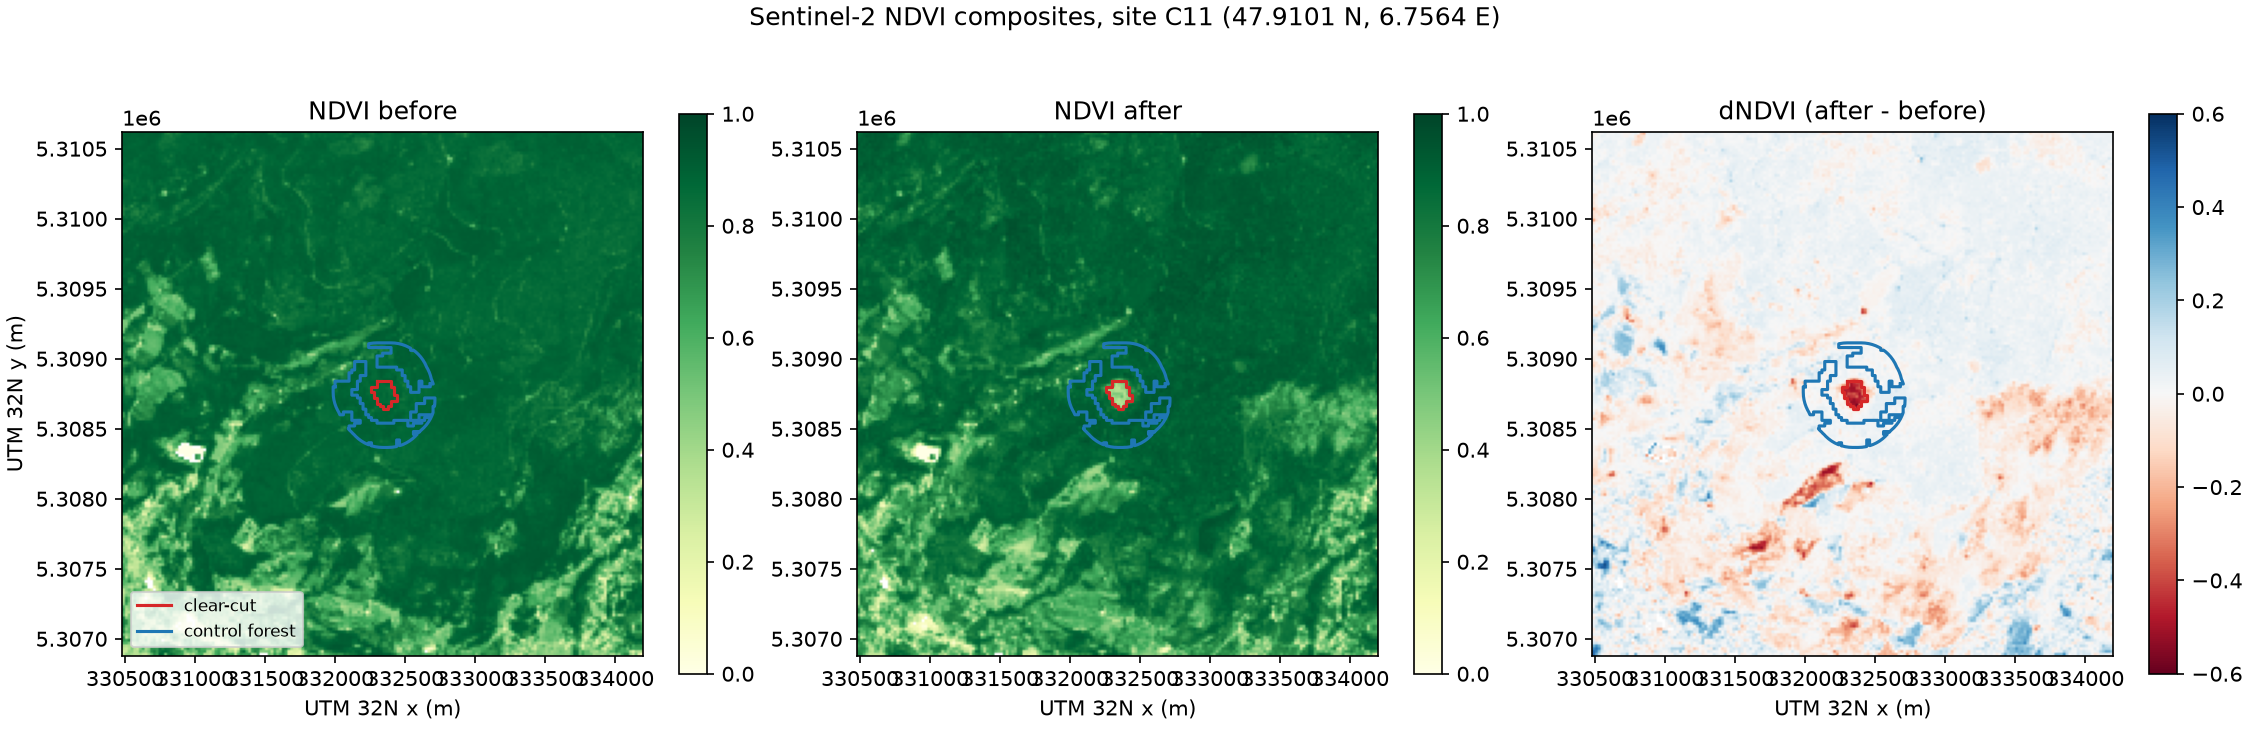
\includegraphics[width=\linewidth,height=0.36\textheight,keepaspectratio]{site_ndvi_maps.png}\\
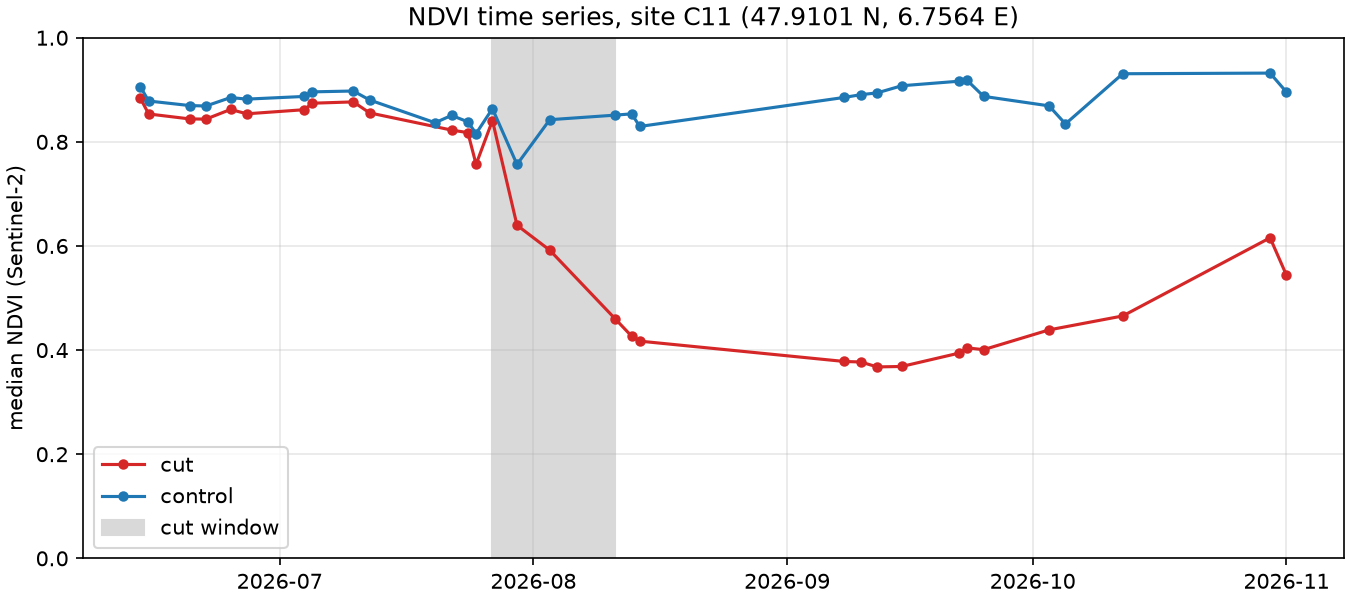
\includegraphics[width=\linewidth,height=0.4\textheight,keepaspectratio]{site_ndvi_timeseries.png}
\column{0.36\textwidth}
\small
\begin{itemize}
\item \textcolor{cut}{\textbf{Coupe}} : 2,36~ha (59 pixels de 20~m), près du Thillot.
\item NDVI 0,84 $\to$ 0,44 : coupe entre le \textbf{27/07 et le 11/08}.
\item \textcolor{ctrl}{\textbf{Témoin}} : anneau de forêt intacte à 100--275~m (548 pixels) : même versant, même
  peuplement, sans effet de lisière.
\end{itemize}
\end{columns}
\end{frame}

%---------------------------------------------------------------------
\section{Méthode}

\begin{frame}{Chaîne de traitement}
\centering
\resizebox{\linewidth}{!}{%
\begin{tikzpicture}[node distance=0.35cm and 0.5cm, every node/.style={font=\scriptsize},
  box/.style={draw, rounded corners, align=center, minimum height=0.85cm, text width=2.45cm},
  arr/.style={-{Latex}, thick}]
\node[box, fill=Lband!15] (n1) {NISAR L2 (ISCE3)\\GCOV + GUNW};
\node[box, fill=Lband!15, right=of n1] (n2) {lecture à distance\\fenêtre du site};
\node[box, fill=Cband!15, below=0.9cm of n1] (s1) {Sentinel-1 SLC\\SAFE réduit (IW2)};
\node[box, fill=Cband!15, right=of s1] (s2) {SNAP : $\gamma^0$ (Terrain-Flattening)\\+ cohérence $10\times3$};
\node[box, fill=gray!15] (g) at ($(n2)!0.5!(s2)+(3.4,0)$) {grille commune\\20~m UTM 32N};
\node[box, fill=gray!15, right=of g] (v) {variables de\\changement};
\node[box, fill=gray!15, right=of v] (m) {AUC, d, JM\\bootstrap blocs};
\node[box, fill=orange!20, below=0.9cm of v] (r) {référence S2\\(dNDVI)};
\node[box, fill=gray!15, right=of r] (d) {prototype de\\détection};
\draw[arr] (n1)--(n2); \draw[arr] (s1)--(s2);
\draw[arr] (n2)--(g); \draw[arr] (s2)--(g); \draw[arr] (g)--(v); \draw[arr] (v)--(m);
\draw[arr] (r)--(d); \draw[arr] (v)--(d);
\end{tikzpicture}}

\vspace{0.6em}
\small
\begin{columns}[T]
\column{0.48\textwidth}
\begin{itemize}
\item Même grandeur des deux côtés : $\gamma^0$ RTC et cohérence à 12~jours.
\item Point technique : site dans un seul burst, donc \textbf{pas d'ESD} (sinon cohérence nulle).
\end{itemize}
\column{0.48\textwidth}
\begin{itemize}
\item Code : paquet \texttt{nisar\_s1} (lecture, SNAP, grille, statistiques, détection, figures) ; 11 tests.
\item Aucun chiffre recopié à la main : les tables LaTeX sont générées.
\end{itemize}
\end{columns}
\end{frame}

\begin{frame}{Protocole d'évaluation}
\begin{columns}[T]
\column{0.5\textwidth}
\textbf{Phases} (fenêtre de coupe 27/07--11/08) :
\begin{itemize}\small
\item \emph{avant} / \emph{après} : images et paires entièrement d'un côté ;
\item \emph{à cheval} : la paire qui encadre la coupe.
\end{itemize}
\textbf{Variables} :
\begin{itemize}\small
\item $\Delta\gamma^0$ = après $-$ avant (dB) ;
\item cohérence de la paire à cheval ;
\item $\Delta$ cohérence après $-$ avant.
\end{itemize}
\column{0.48\textwidth}
\textbf{Métriques} coupe / témoin :
\begin{itemize}\small
\item \textbf{AUC} : probabilité qu'un pixel de coupe soit mieux classé qu'un pixel de forêt (0,5 = hasard ;
  1 = parfait) ;
\item d de Cohen, distance de Jeffries-Matusita ;
\item IC 95~\% par \textbf{bootstrap par blocs} de 60~m (pixels voisins non indépendants) : pas de p-valeurs.
\end{itemize}
\textbf{Garde-fous} :
\begin{itemize}\small
\item \textbf{contrôle avant coupe} : AUC 0,51--0,62, donc témoin valide ;
\item sensibilité : polygones érodés de 20~m.
\end{itemize}
\end{columns}
\end{frame}

%---------------------------------------------------------------------
\section{Résultats}

\begin{frame}{Résultat 1 : la cohérence en bande L voit l'événement de coupe}
\begin{columns}[c]
\column{0.64\textwidth}
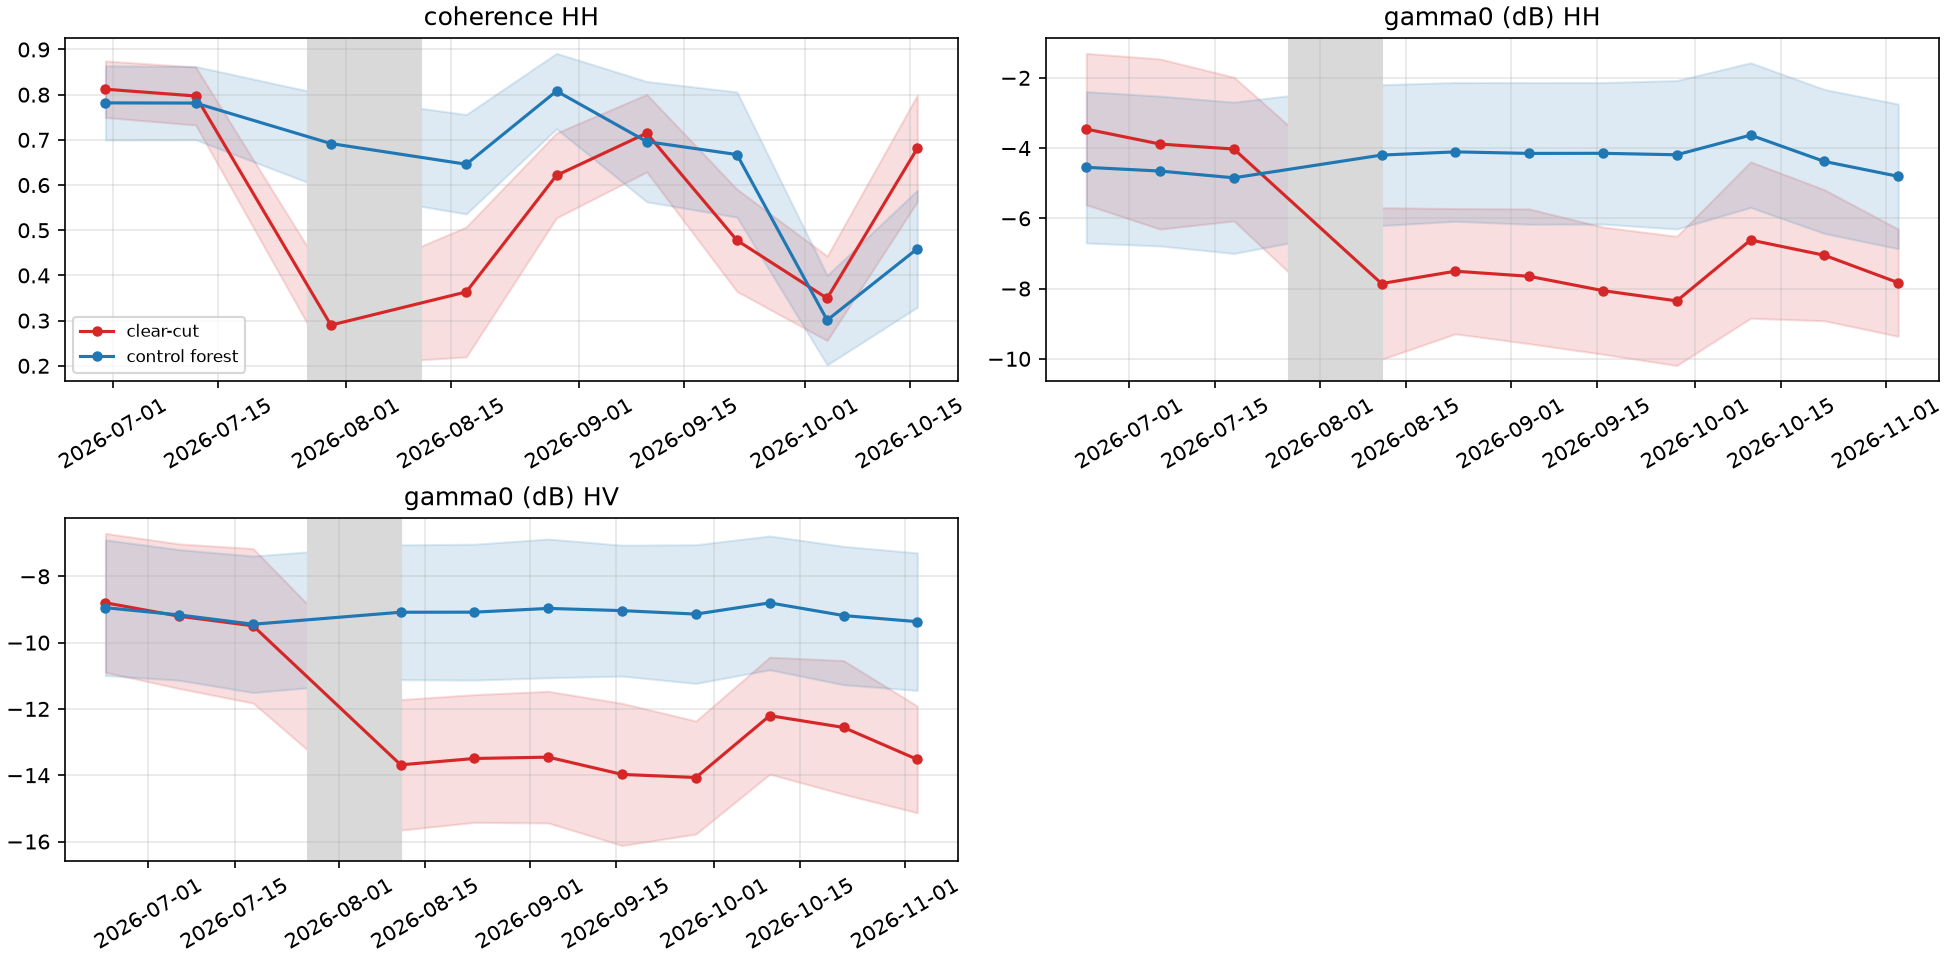
\includegraphics[width=\linewidth]{comparison_ts_NISAR-L_A144F26.png}
\column{0.34\textwidth}
\small
Paire qui encadre la coupe (24~j) :
\begin{itemize}
\item \Lb{L} : coupe 0,29 contre forêt 0,69 : \Lb{AUC 0,995} (A144 et D138).
\item \Cb{C} : coupe 0,23 contre forêt 0,29 : \Cb{AUC 0,74}.
\end{itemize}
Forêt intacte à 12~j : \Lb{0,64--0,70} en L contre \Cb{0,28} en C.

\vspace{0.3em}
\footnotesize En C, la forêt est déjà décorrélée : la coupe n'a « rien à faire chuter ».
\end{columns}
\end{frame}

\begin{frame}{Résultat 2 : la rétrodiffusion baisse dans les deux bandes}
\begin{columns}[c]
\column{0.64\textwidth}
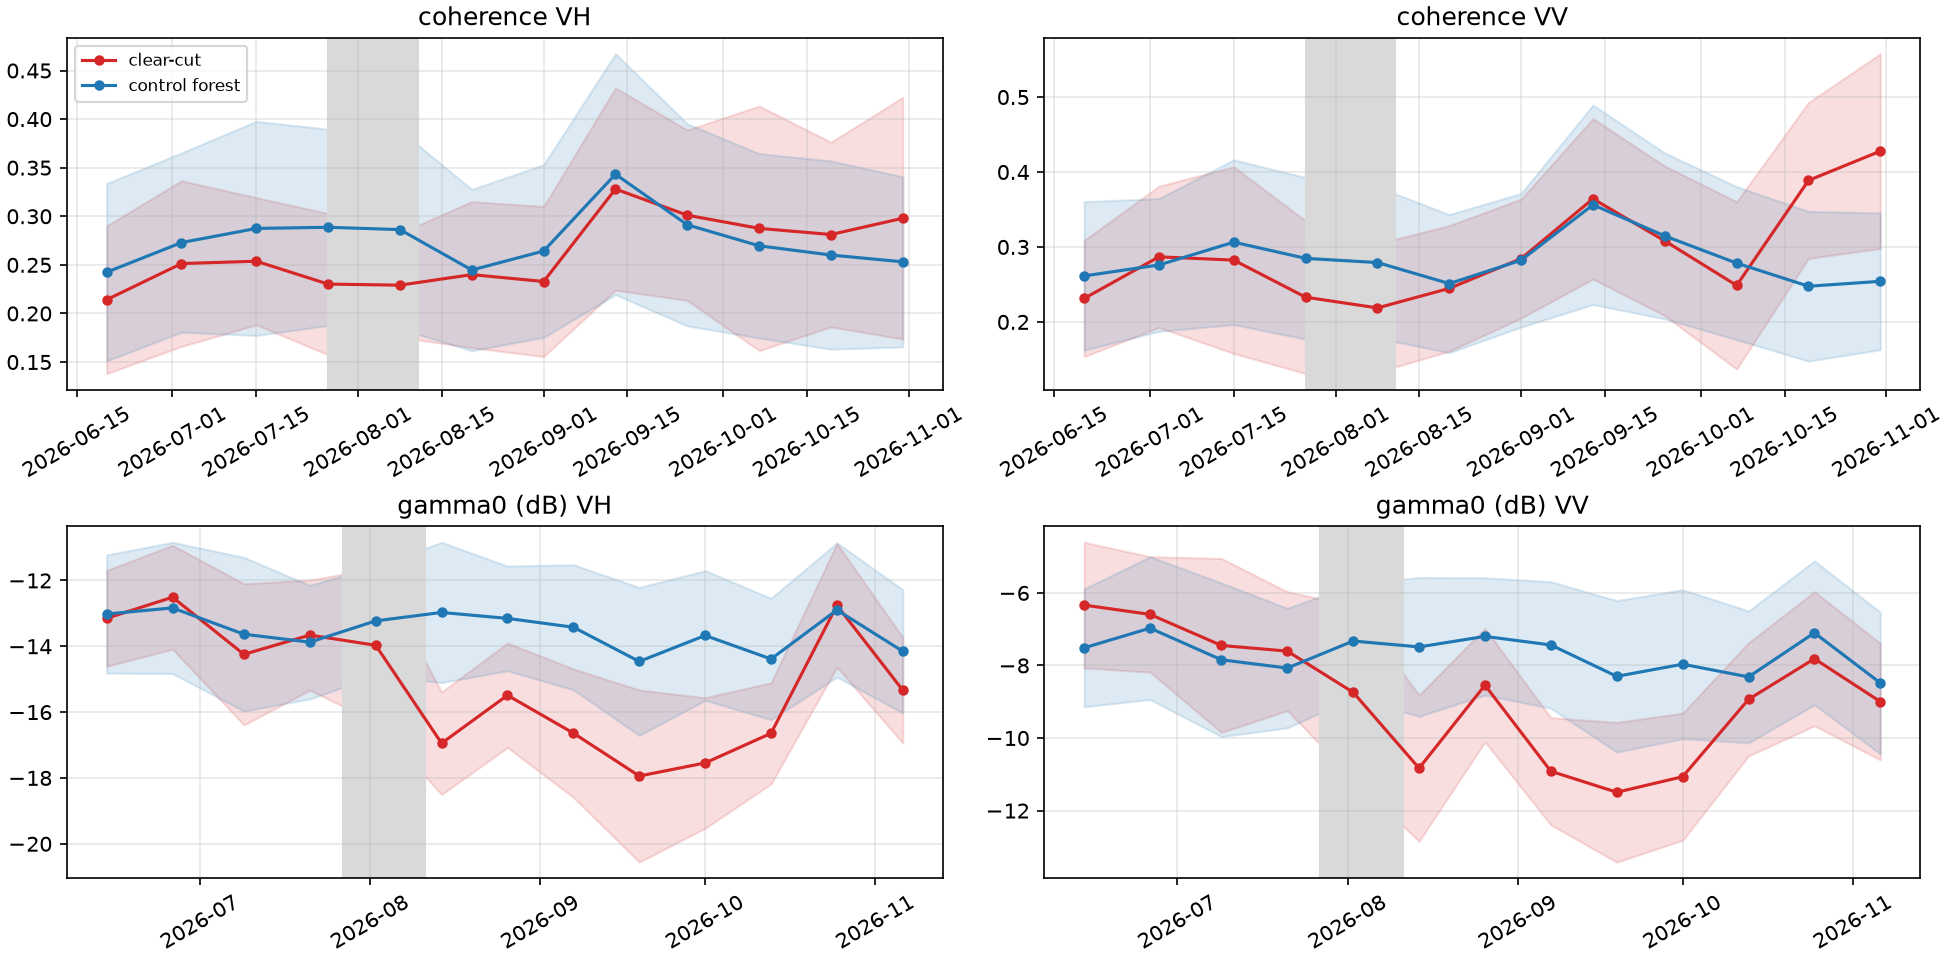
\includegraphics[width=\linewidth]{comparison_ts_S1-C_T139.png}
\column{0.34\textwidth}
\small
Polarisation croisée, après $-$ avant :
\begin{itemize}
\item \Lb{L} A144 : $-4{,}3$~dB, AUC 0,97 ;
\item \Lb{L} A72 : $-3{,}7$~dB, AUC 0,94 ;
\item \Lb{L} D138 : $-2{,}3$~dB, AUC 0,84 ;
\item \Cb{C} D139 : $-2{,}2$~dB, AUC 0,91.
\end{itemize}
\footnotesize En bande C (ci-contre), le contraste s'efface en octobre.
\end{columns}
\end{frame}

\begin{frame}{Résultat 3 : persistance du contraste}
\centering
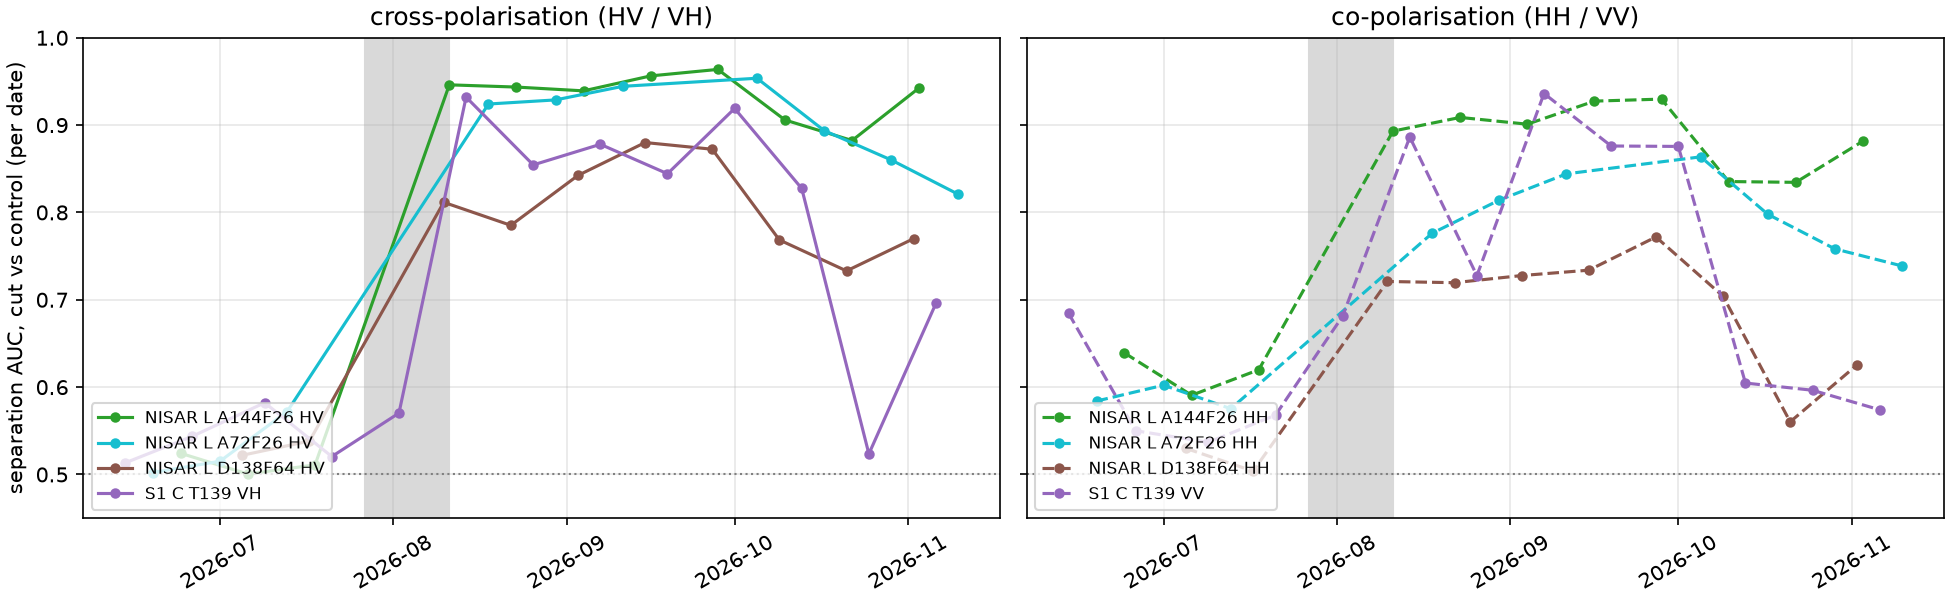
\includegraphics[width=0.92\linewidth]{comparison_persistence.png}

\small AUC date par date. En \Lb{L} montante, le contraste HV reste $\geq 0{,}82$ jusqu'en novembre. En \Cb{C},
il chute en octobre (0,52 le 25/10) : sol nu humide et rémanents rediffusent en bande C.
\end{frame}

\begin{frame}{Cartes de changement}
\centering
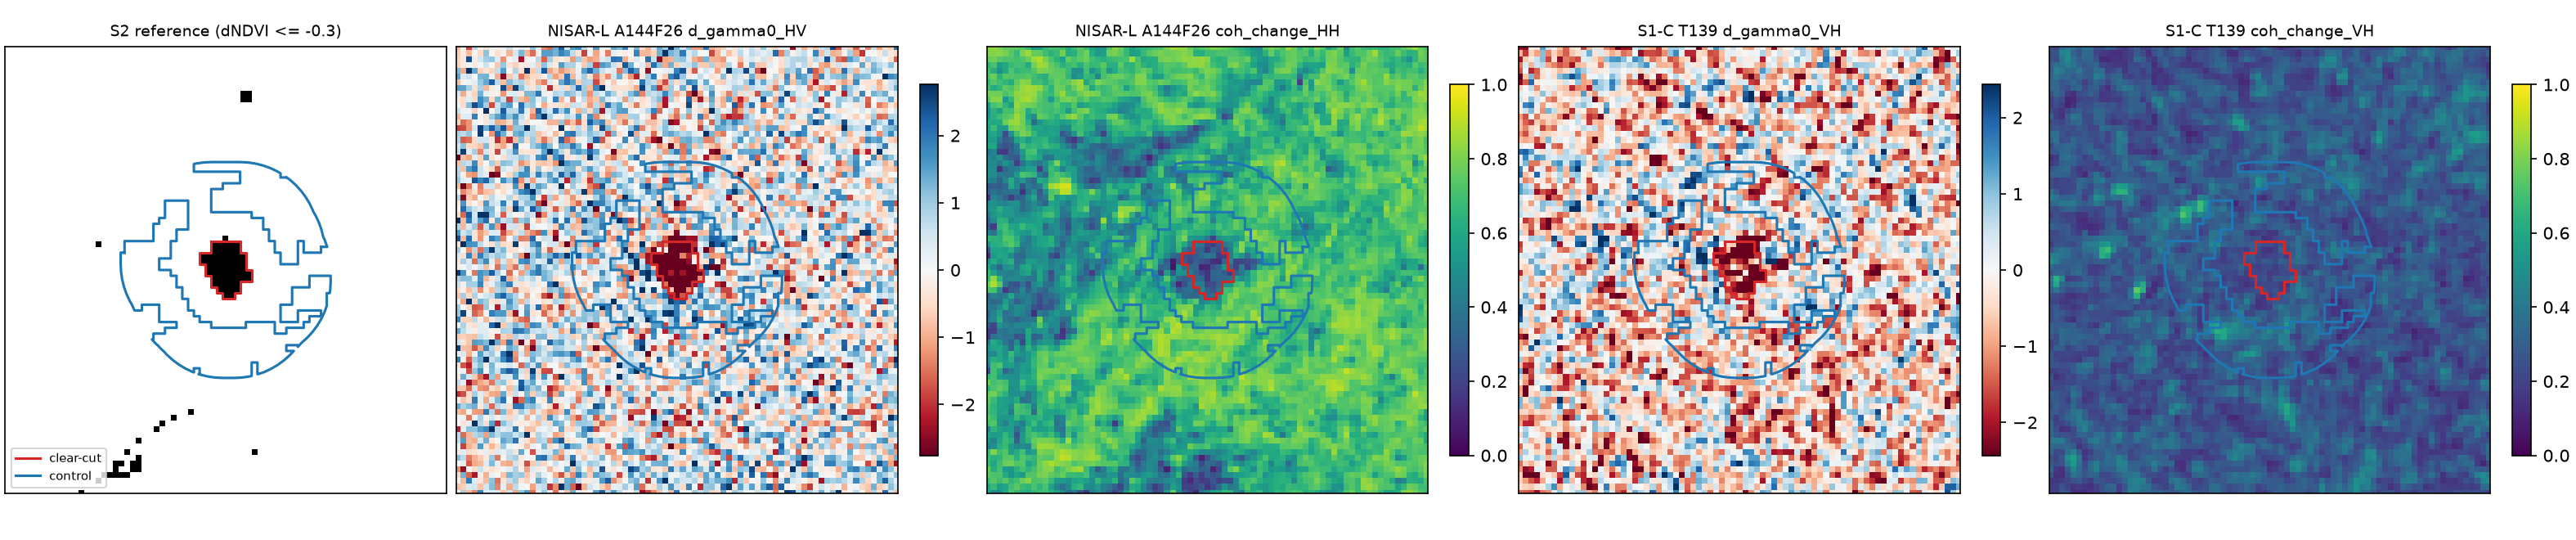
\includegraphics[width=\linewidth]{comparison_maps.png}

\small De gauche à droite : référence S2 ; $\Delta\gamma^0$ HV et cohérence de la paire à cheval
(\Lb{NISAR A144}) ; $\Delta\gamma^0$ VH et cohérence de la paire à cheval (\Cb{Sentinel-1}).
La coupe ressort en cohérence \Lb{L}, pas en cohérence \Cb{C}.
\end{frame}

\begin{frame}{Synthèse honnête : à géométrie égale}
\centering
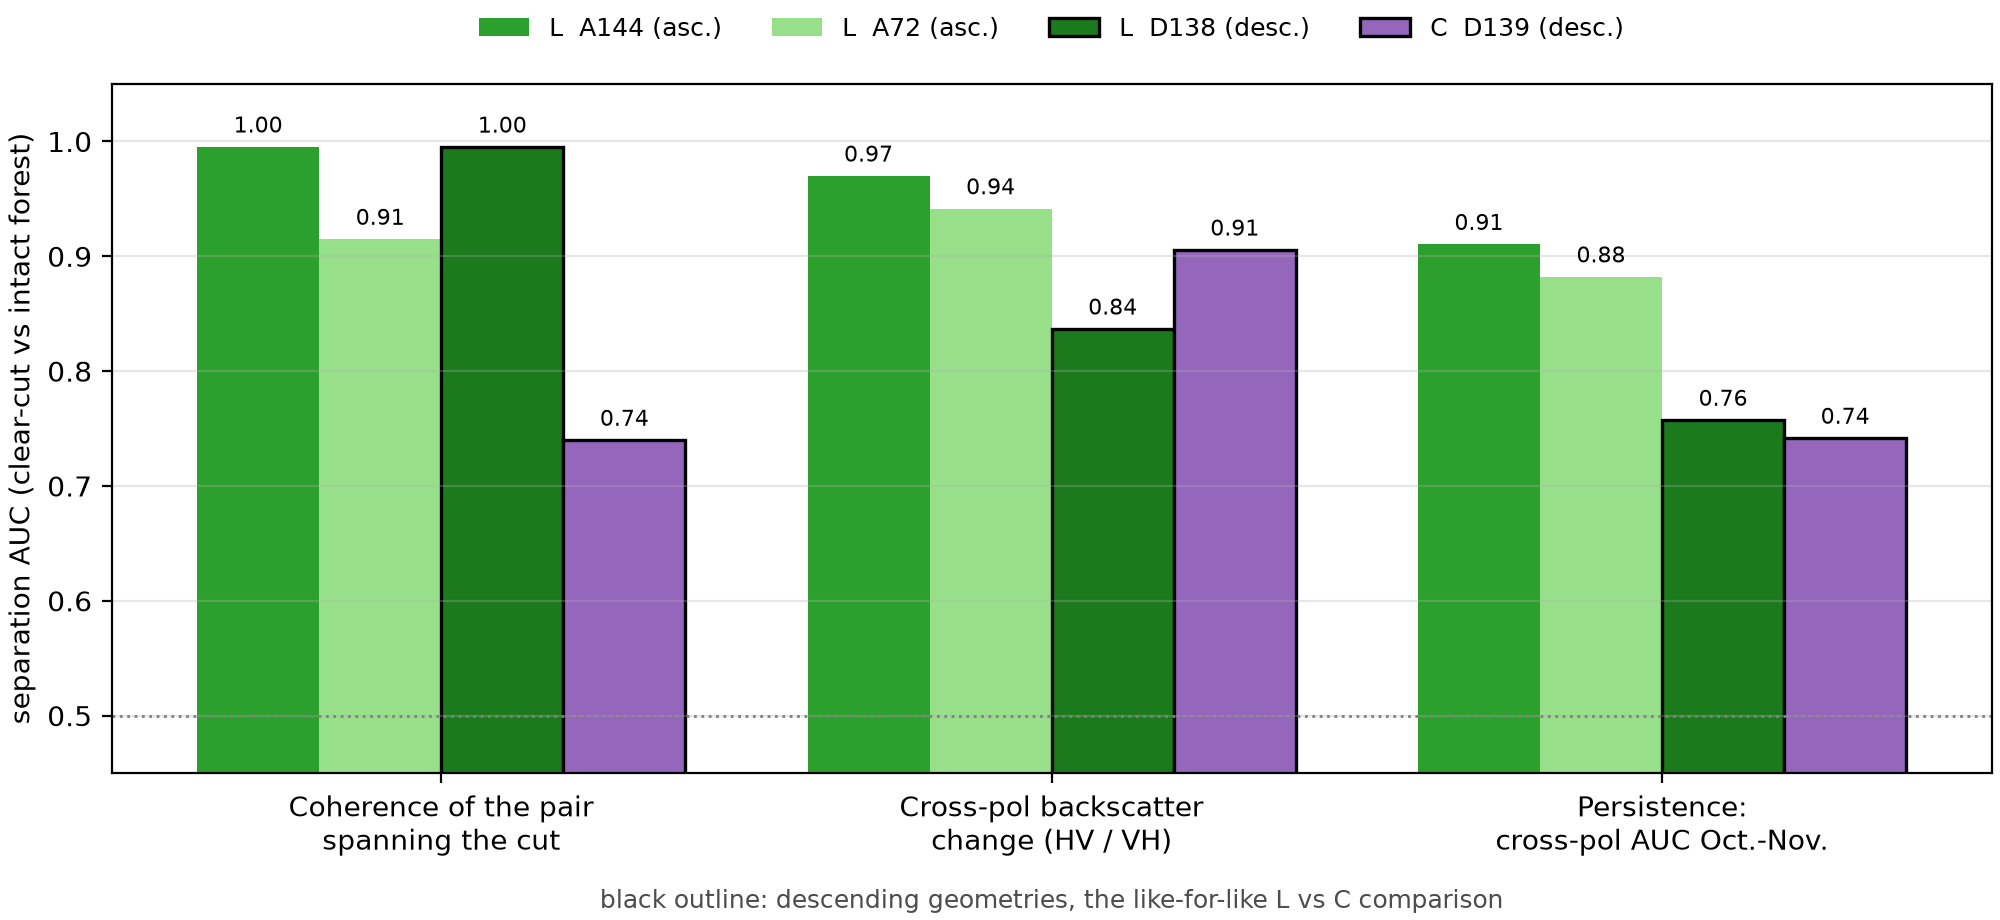
\includegraphics[width=0.84\linewidth]{summary_L_vs_C.png}

\small
\begin{columns}[T]
\column{0.48\textwidth}
\textbf{Robuste} : la \Lb{cohérence L} l'emporte dans les \textbf{trois} géométries (0,91--0,995 contre 0,74).
\column{0.48\textwidth}
\textbf{À nuancer} : en rétrodiffusion, \Lb{L} ne gagne qu'en montante. À géométrie égale (descendante),
\Cb{C} $\approx$ \Lb{L} (0,91 contre 0,84 ; persistance 0,74 contre 0,76).
\end{columns}
\end{frame}

\begin{frame}{Bilan des hypothèses}
\small
\begin{tabular}{@{}lp{9.2cm}l@{}}
\toprule
& Constat sur C11 & Verdict \\
\midrule
H1 & Cohérence de la forêt à 12~j : 0,64--0,70 (L) contre 0,28 (C). À 24~j, encore 0,69 en L. & \Lb{confirmée} \\
H2 & Cohérence de la paire sur la coupe : AUC 0,91--0,995 (L) contre 0,74 (C). & \Lb{confirmée} \\
H3 & $-4{,}3$ / $-3{,}7$~dB (L montante) contre $-2{,}2$~dB (C). En descendante : $-2{,}3$~dB, AUC 0,84 (L) contre
0,91 (C). & \textbf{partielle} \\
H4 & En L, HV $\geq$ HH dans les trois géométries ; mais la cohérence HH fait encore mieux. & \Lb{confirmée} \\
\bottomrule
\end{tabular}

\vspace{0.8em}
\begin{alertblock}{Message scientifique}
L'apport décisif de la bande L sur ce site est \textbf{interférométrique} : en bande L, la forêt reste cohérente,
et une coupe devient un événement nettement visible.
\end{alertblock}
\end{frame}

%---------------------------------------------------------------------
\section{Regard critique}

\begin{frame}{Forces et limites de la démarche}
\begin{columns}[T]
\column{0.48\textwidth}
\textbf{\faCheck\ Forces}
\begin{itemize}\small
\item Hypothèses physiques posées avant les calculs.
\item Référence optique indépendante du radar.
\item Témoin local validé par le contrôle avant coupe.
\item Tailles d'effet et IC par bootstrap par blocs, pas de p-valeurs trompeuses.
\item Sensibilité aux pixels de bord testée.
\item Chaîne entièrement reproductible et versionnée.
\end{itemize}
\column{0.5\textwidth}
\textbf{\faExclamationTriangle\ Limites}
\begin{itemize}\small
\item \textbf{Un seul site} : variabilité inter-sites inconnue.
\item Peu de paires avant la coupe (1--3) ; produits NISAR \emph{provisoires}.
\item Paire L de 24~j contre 12~j en C : défavorable à L, mais aussi un estimateur différent.
\item Effets de géométrie non expliqués (D138 : visée, heure 20~h~42 contre 6~h~19).
\item Cause de la remontée automnale en C supposée (humidité) mais non vérifiée par la météo.
\item F1 de détection faible (0,4~\% de pixels coupés).
\end{itemize}
\end{columns}
\end{frame}

\begin{frame}{Pourquoi le F1 est bas, et ce qu'il faudrait}
\begin{columns}[T]
\column{0.5\textwidth}
\small
\begin{itemize}
\item Sur la fenêtre de $3{,}7\times3{,}7$~km : 95 pixels coupés sur 25\,723 (\textbf{0,4~\%}).
\item AUC de détection élevée (0,82--0,93), mais un seuil sur une seule variable produit plus de fausses
  alarmes que de vrais positifs : \textbf{F1 $\leq$ 0,29}.
\item Ce n'est pas un échec de la bande L : c'est la limite d'un détecteur à un seul seuil, à faible
  prévalence.
\end{itemize}
\column{0.46\textwidth}
\begin{block}{Détecteur réaliste (stage)}
\small
\begin{enumerate}
\item Combinaison de variables : cohérence L et $\gamma^0$ HV (et C pour la réactivité).
\item Plusieurs géométries.
\item Filtre spatial (taille minimale d'objet).
\item Confirmation temporelle (2 dates ou plus).
\end{enumerate}
\end{block}
\end{columns}
\end{frame}

%---------------------------------------------------------------------
\section{Perspectives}

\begin{frame}{Chaîne réutilisable, vers ROSE-L}
\begin{columns}[T]
\column{0.5\textwidth}
\small
\texttt{src/nisar\_s1/} :
\begin{itemize}
\item \texttt{io\_nisar} : lecture des L2 ISCE3, en local ou à distance ;
\item \texttt{download} : extraction partielle ;
\item \texttt{snap} + graphes XML ;
\item \texttt{grid}, \texttt{stats}, \texttt{detect}, \texttt{plots}.
\end{itemize}
Nouveau site = un nouveau GeoJSON.
\column{0.46\textwidth}
\small
\begin{itemize}
\item \textbf{ROSE-L} (2028) : mêmes grandeurs ($\gamma^0$ RTC, cohérence) ; il suffit de remplacer le lecteur.
\item \textbf{ISCE3} est ouvert : on peut produire des L2 équivalents à partir du niveau~1 des deux missions.
\item Complémentarité : C pour \emph{dater} (revisite de 6--12~j, coupe placée entre le 2 et le 11/08), L pour
  \emph{confirmer} et suivre.
\end{itemize}
\end{columns}
\end{frame}

\begin{frame}{Ce que je propose pour le stage}
\begin{enumerate}
\item \textbf{Répliquer} sur d'autres coupes (C09 déjà identifié) et sur des \textbf{dépérissements} (scolytes) :
  la vraie question opérationnelle est de distinguer ces deux phénomènes.
\item \textbf{Expliquer les effets de géométrie} : angle local, orientation versant / visée, heure d'acquisition
  (rosée, vent).
\item \textbf{Détecteur multi-variables} L + C, validé sur une référence indépendante.
\item \textbf{Glissements sous forêt} : la cohérence L conservée en forêt rend possible l'interférométrie de
  déplacement là où la bande C décorrèle (comparaison des GUNW déroulés NISAR et de S1).
\item \textbf{Bande P} (BIOMASS) sur sites tropicaux.
\end{enumerate}
\end{frame}

\begin{frame}[standout]
La bande L garde la forêt \emph{cohérente} :\\
une coupe y devient un \emph{événement} visible.\\[1em]
\normalsize AUC 0,995 en L contre 0,74 en C : un résultat à confirmer sur plusieurs sites,\\
avec une chaîne déjà prête pour ROSE-L.
\end{frame}

%---------------------------------------------------------------------
\appendix
\begin{frame}[fragile]{Annexe : reproduction}
\footnotesize
\begin{verbatim}
python scripts/02_inventory.py               # inventaire ASF
python scripts/03_site_candidates.py         # candidats Sentinel-2
python scripts/03b_verify_candidates.py      # vérification temporelle
python scripts/03c_select_site.py --cand C11 # site et forêt témoin
python scripts/04_fetch_nisar.py             # fenêtres NISAR à distance
python scripts/04_fetch_s1.py --start 2026-06-14 --end 2026-11-07
python scripts/05a_process_s1.py             # SNAP : 13 gamma0 + 12 cohérences
python scripts/05b_compare.py                # comparaison
python scripts/05b_compare.py --erode 20 --tag _erode20
python scripts/06_make_tables.py             # tables LaTeX FR et EN
python scripts/07_summary_figure.py          # figure de synthèse
\end{verbatim}
\normalsize Rapport complet (FR et EN) : \texttt{reports/latex/}.
\end{frame}

\begin{frame}{Annexe : toutes les variables}
\centering
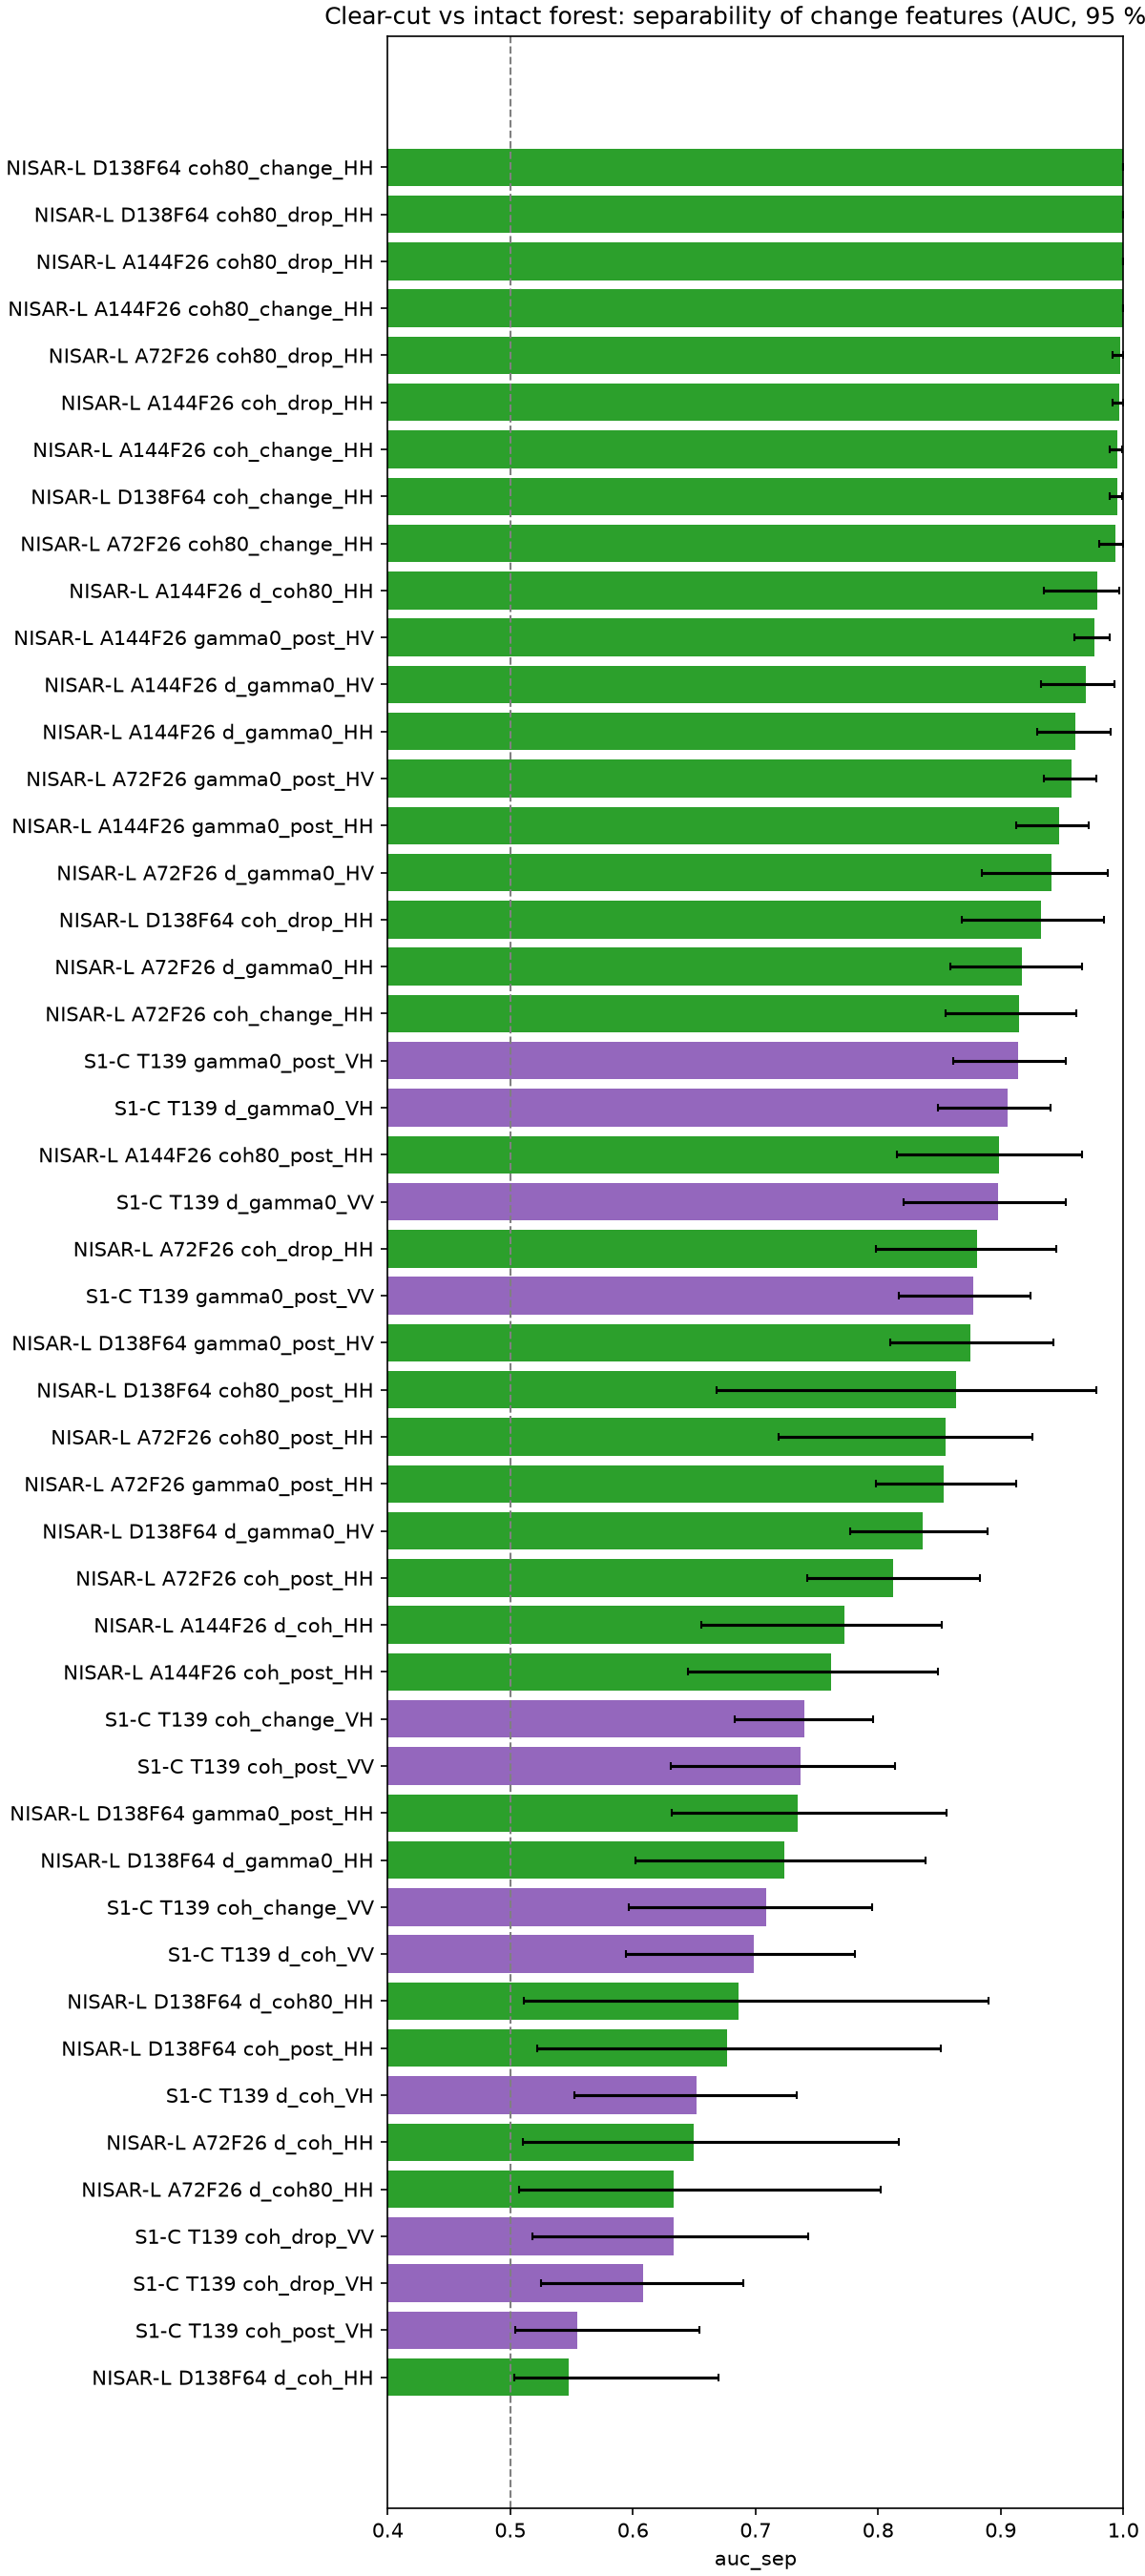
\includegraphics[height=0.86\textheight]{comparison_auc.png}
\end{frame}

\end{document}
